\section{Moduł SIG\_EDR}
\subsection{Badania literaturowe}
		Moduł SIG\_EDR jest odpowiedzialny za wyodrębnienie sygnału oddechu z elektrokardiogramu. Przykładowy przebieg EKG wraz z odpowiadającym mu sygnałem oddechowym zaprezentowany został na Rys.~\ref{fig:ecg_oddech}. Wiedza na temat sposobu oddychania pacjenta jest przydatna przy analizie długoterminowej w celu wykrycia np. bezdechów sennych. Otrzymana w ten sposób informacja nie wymaga użycia dodatkowego sprzętu, mogącego zakłócić naturalny rytm oddechowy.
\begin{figure}[ht]
\centering
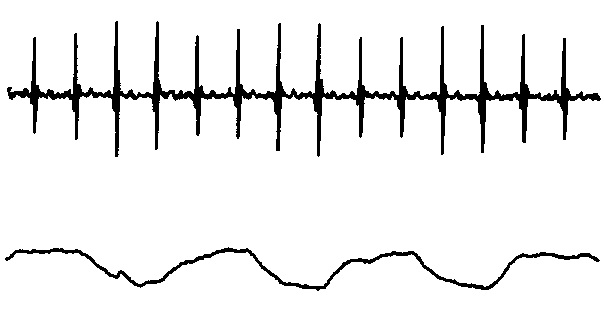
\includegraphics[width=12cm]{SIG_EDR/img/ecg_oddech.jpg}
\caption{EKG (przebieg górny) wraz z sygnałem oddechowym (przebieg dolny)}
\label{fig:ecg_oddech}
\end{figure}
 
		Sposób podejścia do problemu nie zmienił się znacznie w przeciągu lat. Istnieje kilka metod, które zyskały uznanie ze względu na swoją skuteczność tudzież prostotę obliczeniową i łatwość implementacji.
	   
		Pierwszą z nich jest metoda zaproponowana przez Felblinger et al. Polega ona na badaniu amplitudy pików R. Metoda ta wykorzystuje fakt, iż spośród wszystkich faz  EKG piki R podlegają największej modulacji podczas oddychania (w wyniku zmiany impedancji klatki piersiowej). W momencie nabrania powietrza oraz trzymania go w klatce piersiowej jej impedancja rośnie, przez co amplituda pików R maleje, odwrotnie w momencie wydychania – amplituda rośnie. Przekłada się ona zatem bezpośrednio na sposób oddychania. Aby otrzymać ciągły sygnał oddechowy pacjenta należy wykonać interpolację pików R funkcjami sklejanymi (sygnał może zostać poprawnie odtworzony, gdyż prawie zawsze częstość skurczów serca jest przynajmniej dwa razy większa od częstości oddychania – zostaje spełnione twierdzenie o próbkowaniu).  Otrzymany w ten sposób sygnał reprezentuje sposób oddychania pacjenta. Algorytm ten jest łatwy w implementacji oraz dosyć efektywny, wymaga jednak podania dobrze przefiltrowanego sygnału EKG na wejście (niezwykle istotna jest eliminacja falowania izolinii).
	   
		Kolejna metoda również opiera się na badaniu pików R. Tutaj jednak liczony jest czas trwania fali R. W tym celu w pierwszej kolejności liczona jest pochodna sygnału EKG w oknie czasowym o długości 40 ms (+/- 20 ms od piku R). Pochodna ta generuje jedno minimum oraz jedno maksimum lokalne (dla danego piku R). Wartości różnic czasowych pomiędzy minimum a maksimum umieszcza się na wykresie w funkcji czasu wystąpienia danego piku R. Następnie otrzymane punkty interpoluje się funkcjami sklejanymi, otrzymując w ten sposób sygnał EDR. Obie przytoczone metody zostały porównane w pracy Murtaza M. Lakdawala „Derivation of the respiratory rate signal from a single lead ECG”. Została w niej również zaprezentowana metoda łącząca wyniki otrzymane z obu metod.
	   
		Jedną z bardziej znanych metod jest ta zaproponowana przez Moody et al. Wykorzystuje ona sygnał z dwóch odprowadzeń. Metodę tą, podobnie jak poprzednie, realizuje się na odfiltrowanym sygnale EKG. Sygnał oddechu wyznaczany jest na podstawie zmiany kąta nachylenia głównego wektora sercowego w stosunku do osi jednego z wyprowadzeń. W celu wyznaczenia takiego wektora należy obliczyć pole powierzchni wartości bezwzględnej z kompleksów QRS dla każdego z wyprowadzeń. Następnie, aby wyznaczyć poszukiwane nachylenie, należy obliczyć arctg ze stosunku obu otrzymanych powierzchni (Rys.~\ref{fig:moody_alg}). W ten sposób dla każdego kompleksu QRS otrzymujemy jedną wartość nachylenia głównego wektora sercowego. Aby wygenerować ciągły sygnał oddechowy należy otrzymane punkty interpolować funkcjami sklejanymi. Algorytm ten zakłada ortogonalność wyprowadzeń. Jeżeli jednak warunek ten nie jest spełniony to generowany jest stały błąd, który nie ma znaczącego wpływu na wyznaczanie nachylenia głównego wektora sercowego.
	   
\begin{figure}[ht]
\centering
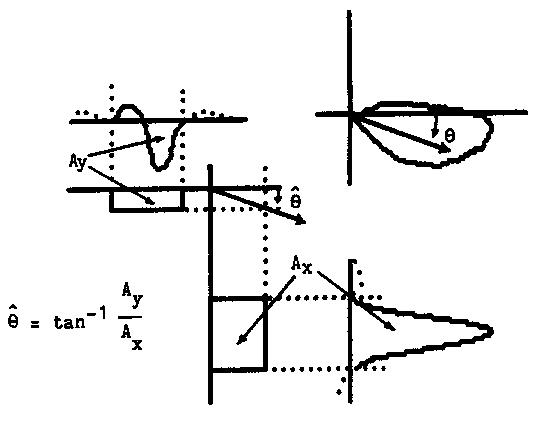
\includegraphics[width=12cm]{SIG_EDR/img/moody_alg.jpg}
\caption{Sposób wyznaczania nachylenia głównego wektora sercowego od osi jednego z wyprowadzeń.}
\label{fig:moody_alg}
\end{figure}
\newpage
		Istnieją również algorytmy wykorzystujące większą liczbę wyprowadzeń. Nie zostały one jednak rozpatrzone, ze względu na wykorzystanie w projekcie jedynie dwóch wyprowadzeń.
	   
 
\subsection{Koncepcja proponowanego rozwiązania}
 
		Z racji stosunkowo niewielkiego poziomu skomplikowania algorytmów zdecydowano się na implementację dwóch spośród wymienionych, tj. pierwszego (analiza amplitudy pików R) oraz ostatniego (badanie odchylenia głównego wektora sercowego od osi jednego z wyprowadzeń) celem porównania działania.
	   
		W przypadku pierwszego algorytmu zostały wykorzystane informacje pochodzące z modułu odpowiedzialnego za wykrywanie pików R (R\_PEAKS). Moduł ten wysyła indeksy próbek, dla których został wykryty pik R. Wartości sygnału z próbek o zadanych indeksach są następnie  interpolowane metodą funkcji sklejanych. Rząd wielomianu determinowany jest na podstawie najlepszego dopasowania do interpolowanego sygnału.   Otrzymana za pomocą interpolacji krzywa stanowi sygnał oddechowy.
 
		Drugi algorytm wykorzystuje informacje pochodzące z modułu odpowiedzialnego za detekcję punktów charakterystycznych sygnału EKG (WAVES). Schemat blokowy algorytmu został przedstawiony na poniższym rysunku (Rys.~\ref{fig:graf}):
	   
\begin{figure}[ht]
\centering
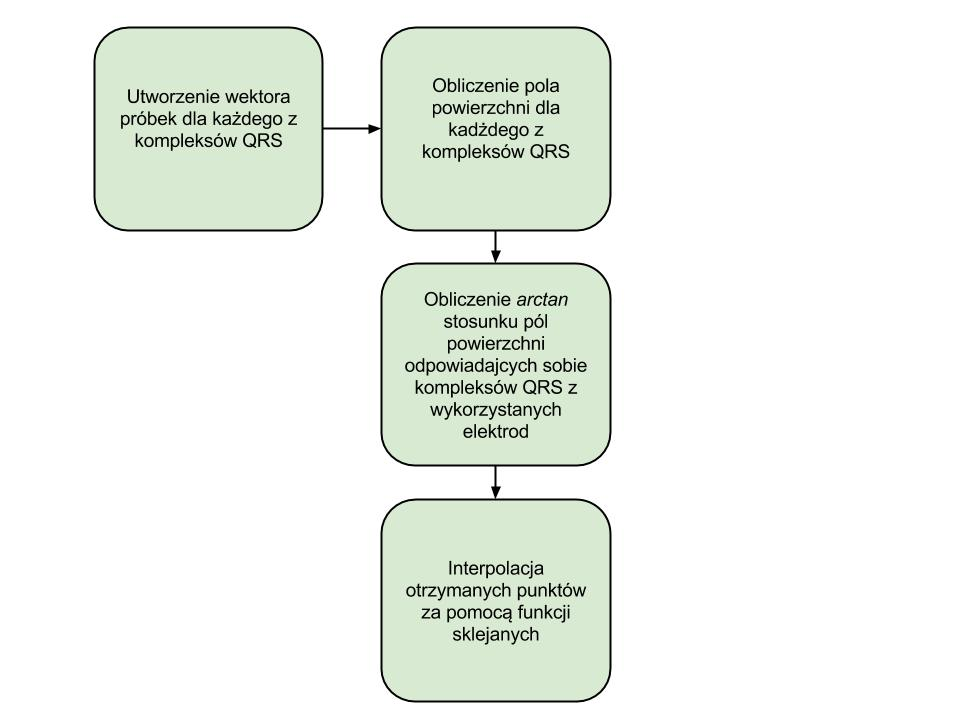
\includegraphics[width=12cm]{SIG_EDR/img/graf.jpg}
\caption{Schemat blokowy realizujący odczytywanie sygnału EDR z wykorzystaniem modułu WAVES}
\label{fig:graf}
\end{figure}   
	   
		 Na podstawie otrzymanych punktów QRSonset oraz QRSend wyznaczane jest pole powierzchni każdego z kompleksów QRS, zarówno z pierwszej, jak i z drugiej elektrody. Pole powierzchni kompleksu jest proporcjonalne do średniej amplitudy sygnału. Zakładając ortogonalność osi wyprowadzeń, $\arctan$ ze stosunku pól powierzchni obu kompleksów daje w wyniku kąt odchylenia głównego wektora sercowego od jednej z osi wyprowadzeń. Jeżeli wyprowadzenia nie są ortogonalne pojawia się błąd pomiaru. Jest on jednak stały dla całego sygnału i nie ma wpływu na wyznaczanie sygnału oddechu pacjenta.
 
		Obie metody charakteryzują się wysoką dokładnością odtwarzania sygnału oddechowego. Nie wymagają wykonywania dużej ilości obliczeń oraz są stosunkowo proste w implementacji. Dodatkową zaletą pierwszej z nich jest wykorzystanie do obliczeń sygnału z jednego odprowadzenia.
	   
\subsection{Rezultaty i wnioski}
 
		Działanie modułu zostało przedstawione na poniższych obrazkach (Rys.~\ref{fig:aplikacja_1}) oraz Rys.~\ref{fig:aplikacja_2}).
	   
\begin{figure}[h]
\centering
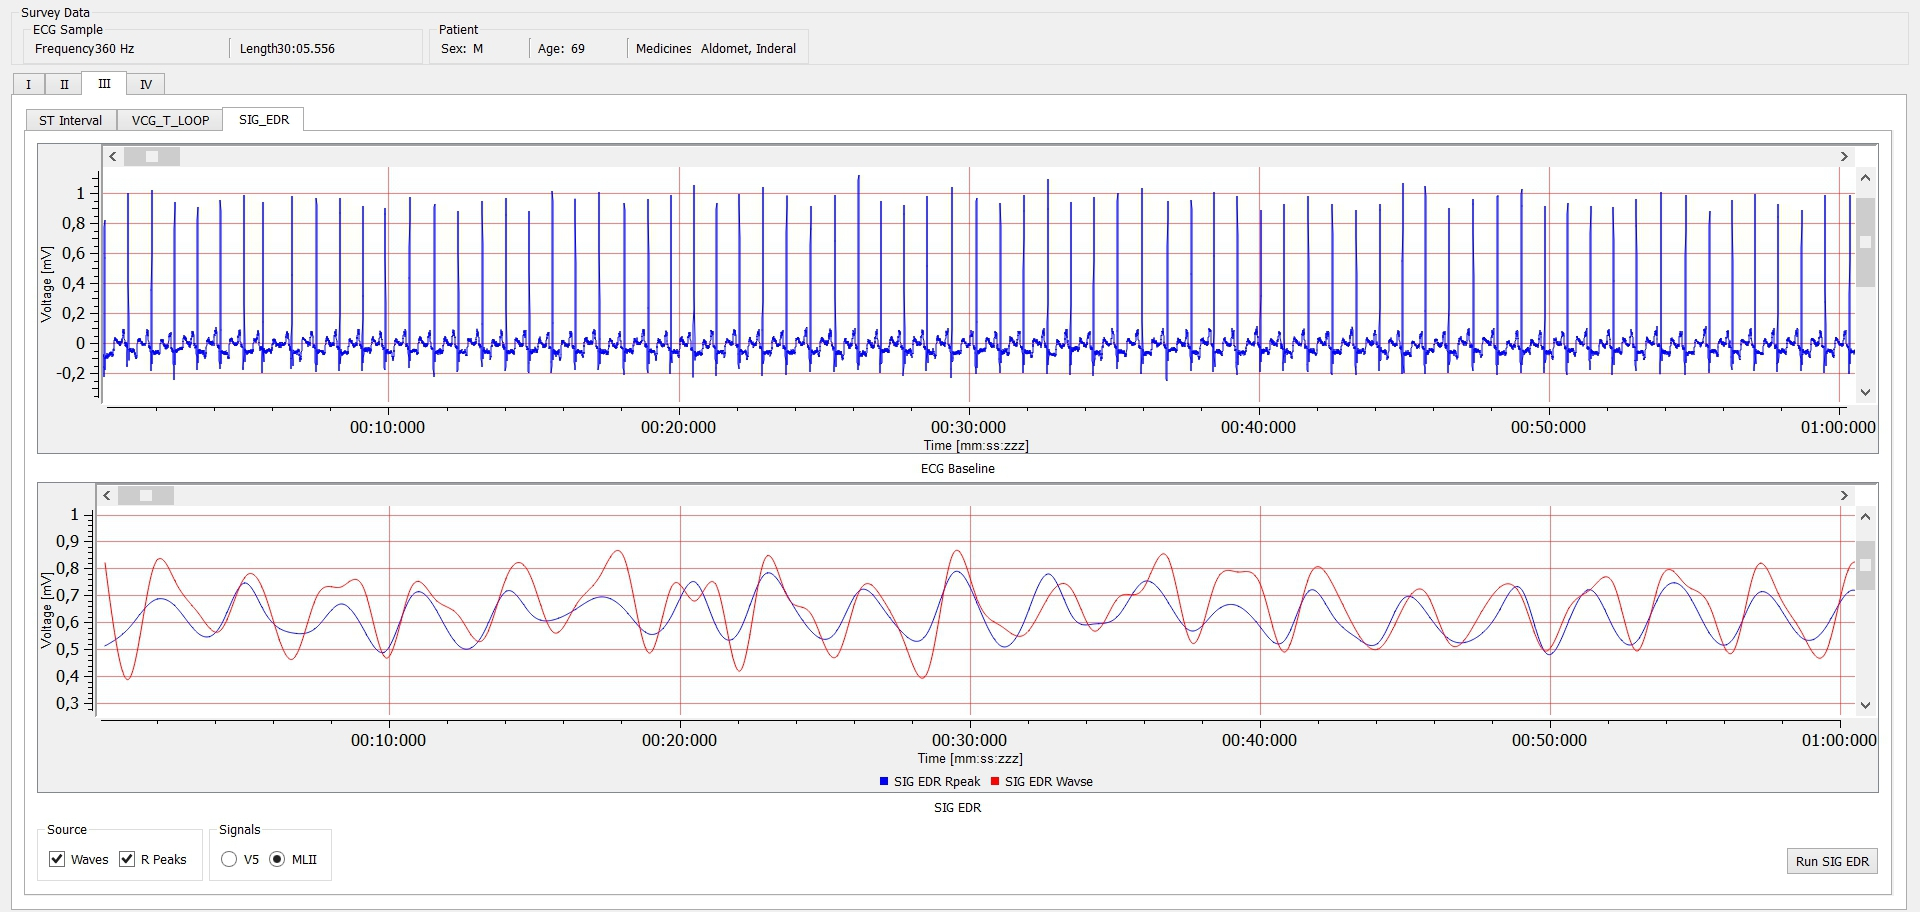
\includegraphics[width=12cm]{SIG_EDR/img/aplikacja_1_1.jpg}
\caption{Działanie modułu dla rekordu 100, pierwsza minuta sygnału}
\label{fig:aplikacja_1}
\end{figure}
 
\begin{figure}[h]
\centering
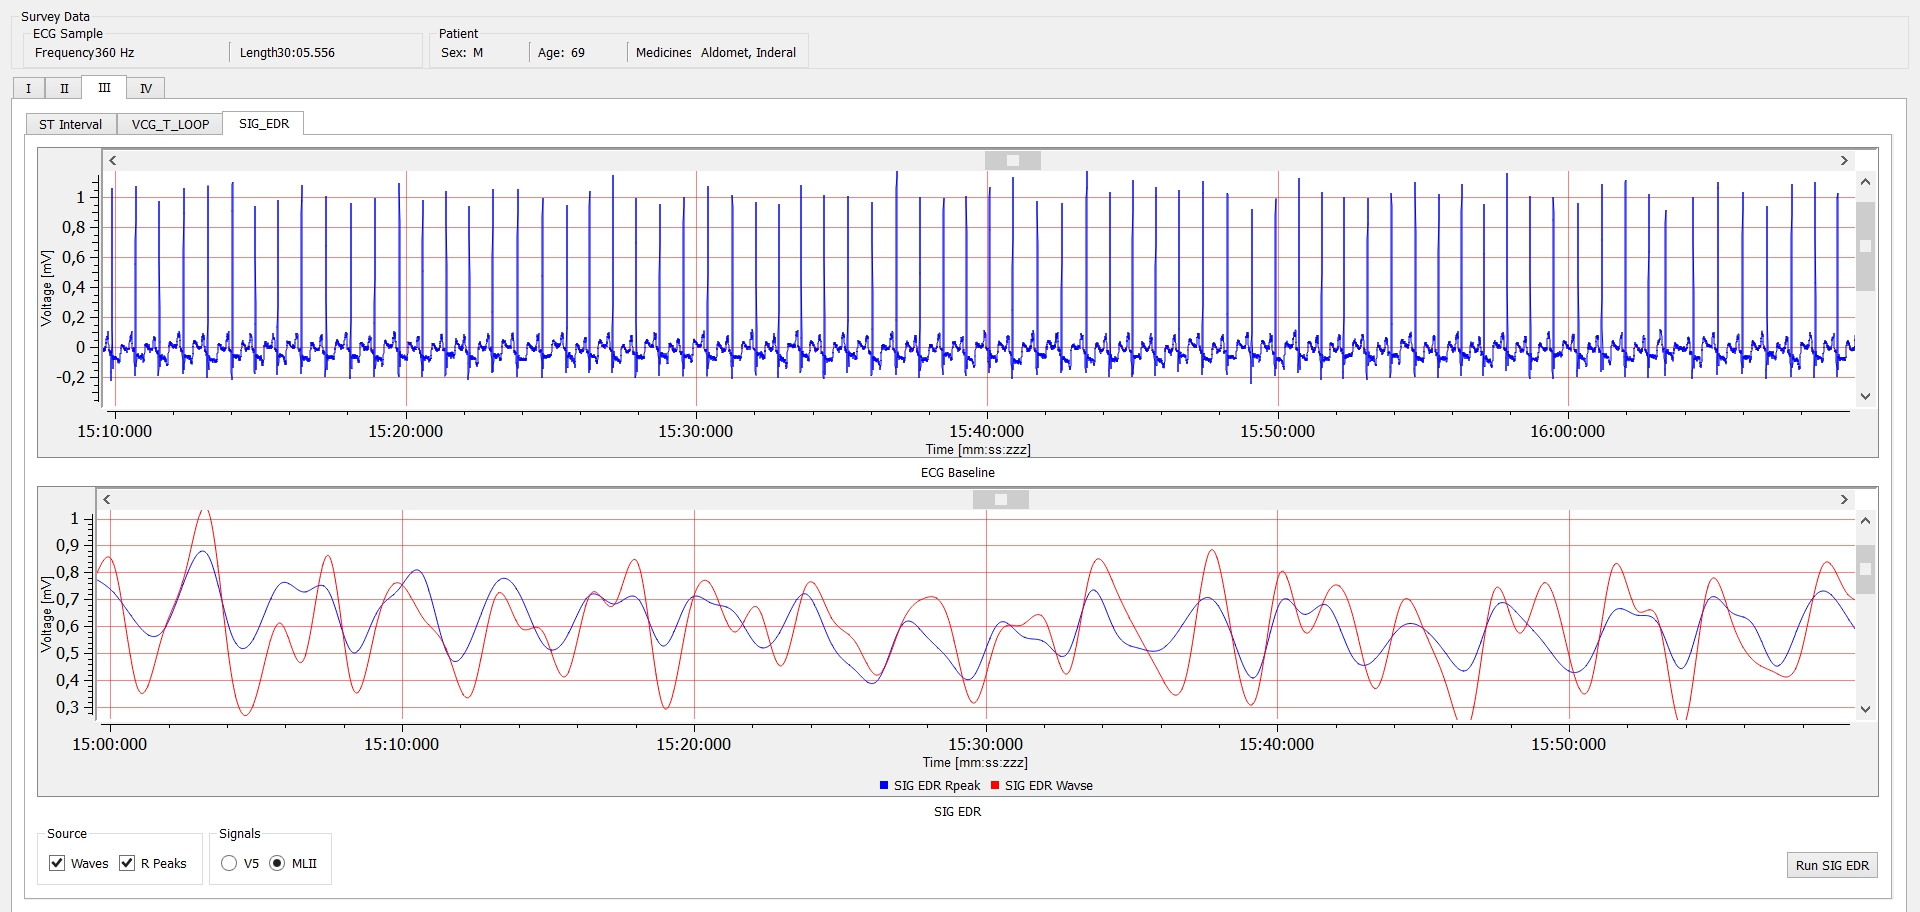
\includegraphics[width=12cm]{SIG_EDR/img/aplikacja_2_2.jpg}
\caption{Działanie modułu dla rekordu 100, piętnasta minuta sygnału}
\label{fig:aplikacja_2}
\end{figure}
 
		Niestety, z braku dostępu do rzeczywistego sygnału oddechowego dla posiadanych danych, przebiegi nie mogły zostać porównane w sposób analityczny. Jedynym sposobem sprawdzenia poprawności otrzymanego sygnału EDR było porównanie kształtu przebiegu z sygnałem ECG, a następnie porównanie z wzorcowymi sygnałami, uzyskanymi przy pomocy aparatury do mierzenia oddechu (PRT). Z tej przyczyny skupiono się na przeprowadzeniu porównania otrzymanych danych w celu weryfikacji poprawności zastosowanych algorytmów.
	   
		Dane zostały porównane w następujący sposób:
		\begin{itemize}
		\item obliczenie różnicy pomiędzy wartościami próbek stanowiących R-piki z wartościami                                   otrzymanymi w wyniku działania modułu
		\item porównanie wartości zwracanych w wyniku zastosowania drugiego algorytmu (Moody) z                               wartościami uzyskanymi z poprzedniego algorytmu
		\item obliczenie odchylenia poszczególnych różnic od średniej różnicy badanego przebiegu                          (odchylenie standardowe)
		\end{itemize}
	   
		Obliczone wartości zostały zgromadzone w tabeli zbiorczej(Tab. ~\ref{tabela_wynikow}). \newline
 
\begin{table}[ht]
\centering
\begin{tabular}{|c|c|c|c|c|c|c|c|c|c|}
\hline
	R1 & R2 & QRS & RR1 & R1Q & R2Q & WR1 & WR2 & WR3\\
\hline
		0,514&0,774&0,822&-0,260&-0,307&-0,047&0,554&0,340&0,308\\
		0,580&0,951&0,392&-0,371&0,188&0,559&0,665&0,155&0,298\\
		0,678&0,960&0,797&-0,282&-0,120&0,163&0,576&0,153&0,098\\
		0,658&0,903&0,747&-0,246&-0,090&0,156&0,540&0,123&0,105\\
		0,557&0,911&0,632&-0,354&-0,075&0,279&0,648&0,108&0,018\\
		0,591&0,888&0,572&-0,297&0,019&0,316&0,591&0,014&0,055\\
		0,747&0,991&0,769&-0,244&-0,022&0,222&0,538&0,055&0,039\\
		0,643&0,921&0,713&-0,278&-0,070&0,208&0,572&0,104&0,053\\
		0,563&0,948&0,466&-0,385&0,097&0,482&0,679&0,064&0,221\\
		0,581&0,909&0,699&-0,328&-0,118&0,210&0,622&0,151&0,051\\
		0,670&0,933&0,733&-0,263&-0,063&0,200&0,557&0,096&0,061\\
		0,571&0,878&0,723&-0,307&-0,152&0,155&0,601&0,185&0,106\\
		0,494&0,861&0,468&-0,367&0,026&0,392&0,661&0,007&0,132\\
		0,695&0,936&0,728&-0,241&-0,032&0,208&0,535&0,066&0,052\\
		0,652&0,908&0,685&-0,256&-0,033&0,223&0,550&0,067&0,038\\
		0,512&0,849&0,623&-0,337&-0,111&0,226&0,631&0,144&0,035\\
		0,557&0,919&0,536&-0,362&0,021&0,383&0,656&0,012&0,122\\
		0,718&0,957&0,774&-0,239&-0,056&0,183&0,533&0,089&0,078\\
		0,634&0,881&0,775&-0,247&-0,141&0,106&0,541&0,174&0,155\\
		0,609&0,901&0,564&-0,293&0,045&0,337&0,587&0,011&0,076\\
		0,649&0,965&0,664&-0,316&-0,015&0,301&0,610&0,048&0,041\\
		0,693&0,908&0,772&-0,215&-0,078&0,136&0,509&0,111&0,125\\
		0,647&0,883&0,832&-0,236&-0,185&0,050&0,530&0,219&0,210\\
		0,558&0,929&0,486&-0,371&0,073&0,443&0,665&0,039&0,182\\
		0,626&0,935&0,734&-0,310&-0,108&0,202&0,604&0,141&0,059\\
		0,751&0,959&0,680&-0,208&0,072&0,280&0,502&0,039&0,019\\
		0,581&0,897&0,733&-0,317&-0,153&0,164&0,611&0,186&0,097\\
		0,571&0,929&0,421&-0,358&0,151&0,509&0,652&0,117&0,248\\
		0,777&0,963&0,826&-0,186&-0,049&0,137&0,480&0,082&0,124\\
		0,703&0,911&0,697&-0,208&0,006&0,214&0,502&0,027&0,047\\
		0,567&0,915&0,632&-0,348&-0,065&0,283&0,642&0,098&0,022\\
		0,564&0,968&0,472&-0,404&0,092&0,496&0,698&0,059&0,235\\
		0,716&0,993&0,711&-0,278&0,005&0,282&0,572&0,029&0,021\\
		0,659&0,950&0,690&-0,291&-0,032&0,259&0,585&0,065&0,001\\
 
\hline
\end{tabular}
\caption{Porównanie wartości próbek R-pików z obu elektrod oraz metody wykorzystującej moduł WAVES.
			R1 - wartości próbek z pierwszej elektrody, R2 - wartości próbek z drugiej elektrody, QRS - wartości próbek otrzymanych metodą wykorzystującą moduł WAVES, RR1 - różnice pomiędzy wartościami odpowiadających próbek z R1 i R2, R1Q - różnice pomiędzy wartościami odpowiadających próbek z R1 i QRS, R2Q - różnice pomiędzy wartościami odpowiadających próbek z R2 i QRS, WR1, WR2, WR3 - odchylenia od średniej różnicy dla kolejnych par (odpowiednio RR1, R1Q oraz R2Q) }
\label{tabela_wynikow}
\end{table}
	   
 
		Przeprowadzone badania miały na celu sprawdzenie czy kształt sygnału oddechowego jest taki sam dla każdej z zastosowanych metod. Badana różnica pomiędzy poszczególnymi sygnałami EDR powinna być zatem stała, bądź jak najbardziej zbliżona do stałej. Wynika to z faktu, iż w rzeczywistości mamy do czynienia z jednym sygnałem oddechowym, który jest taki sam dla każdej z zastosowanych metod. Niezależnie od zastosowanej metody, wyniki powinny mieć podobny kształt, mogą się jednak różnić wartościami, wynikającymi z różnych odległości elektrod od serca, a tym samym mocą sygnału. Na wykresie skutkuje to wertykalnym przesunięciem przebiegu i jego lekką deformacją.
	   
		Kształt przebiegu sygnału EDR w niewielkim stopniu odbiega od kształtu sygnałów wzorcowych, otrzymanych z pneumatycznej aparatury pomiarowej. Głównymi czynnikami generującymi różnice pomiędzy sygnałami EDR są nienaturalne różnice występujące pomiędzy badanymi próbkami, a tym samym wykrytymi pikami R, które są filarem stosowanego algorytmu. Podobne problemy występują w przypadku drugiego z algorytmów, gdyż jest on zależny od obu próbek. Dodatkowo nie wszystkie wykryte obszary QRS, z których ten algorytm korzysta, są poprawne.
	   
\subsection{Diagram klasy}
\begin{tikzpicture}
%       \begin{class}[text width = 9cm]{sig_edr}{0,0}
%               \attribute{+ signal_one; : const QVector<double>}
%               \attribute{+ signal_two :const QVector<double>}
%               \attribute{+ EDRsignal_RPeaks_one : QVector<double> }
%               \attribute{+ EDRsignal_RPeaks_two : QVector<double>}
%               \attribute{+ EDRsignal_Waves : QVector<double>}
%               \attribute{+ EDRsignal : std::vector<double>}
%               \attribute{+ Integrals_one :  QVector<double>}
%               \attribute{+ Integrals_two :  QVector<double>}
%              
%               \operation{+ sig_edr(\&signal_one : const QVector<double>,\\
%                       \&signal_two : const QVector<double>)}
%               \operation{+ sig_edr(\&signal_one : const QVector<double>,\\
%                       \&signal_two : const QVector<double>,\\
%                       \&RPeaksIterators_one : const QVector<unsigned int>,\\
%                       \&RPeaksIterators_two : const QVector<unsigned int>)}
%               \operation{+ sig_edr(\&signal_one : const QVector<double>,\\
%                       \&signal_two : const QVector<double>,\\
%                       \&QRSonsetIterators_one : const vector_it,\\
%                       \&QRSonsetIterators_two : const vector_it,\\
%                       \&QRSendIterators_one : const vector_it,\\
%                       \&QRSendIterators_two : const vector_it)}
%               \operation{+ new_RPeaks_signal(\&signal_num : int,\\
%                       \&RPeaksIterators : const QVector<unsigned int>) : void}
%               \operation{+new_Waves_signal(\&QRSonsetIterators_one : const vector_it,\\
%                       \&QRSonsetIterators_two : const vector_it,\\
%                       \&QRSendIterators_one : const vector_it,\\
%                       \&QRSendIterators_two : const vector_it) : void}
%               \operation{+ retrieveEDR_QVec(\EDR_type : int,\\
%                       \&signal_num : int) : QVector<double>*}
%               \operation{+ retrieveEDR_StdVec(\EDR_type : int,\\
%                       \&signal_num : int) : std::vector<double>*}
%               \operation{- integral( &value : QVector<double>) : double}
%               \operation{- calculate_signal_from_QRS(\&QRSIntegrals_one : const QVector<double>,\\
%                       \&QRSIntegrals_two : const QVector<double>) : void}
%       \end{class}
%      
 
\end{tikzpicture}

